\subsection{Selective content edits discriminate direction from source}

Selective edits distinguished direction from source, despite a whole-permutation response to both cues. Direction signs and arbitrary Cedar/Maple source cues were generated independently in twenty irregular worlds per target mechanism. Targets depended on direction, source or available-note count alone. Each edit retained the alternative cue within the finite test vocabulary (Table~\ref{tab:construct_examples}).

\begin{table}[htbp]
\centering\small
\caption{One paired example from the frozen construct configuration's test and paraphrase templates. Each selective edit changes one stipulated cue while retaining the other; the paraphrase retains both. Targets and the event process remain fixed.}
\label{tab:construct_examples}
\begin{tabular}{@{}>{\raggedright\arraybackslash}p{0.18\linewidth}>{\raggedright\arraybackslash}p{0.78\linewidth}@{}}
\toprule
Condition & Text at the same event slot\\
\midrule
Aligned & We predict that demand will increase in the upcoming interval. Bulletin source: Cedar.\\
Direction flip & We predict that demand will decrease in the upcoming interval. Bulletin source: Cedar.\\
Source flip & We predict that demand will increase in the upcoming interval. Bulletin source: Maple.\\
Paraphrase & An increase in demand is forecast for the interval ahead. Bulletin source: Cedar.\\
\bottomrule
\end{tabular}
\end{table}


Whole permutation, implemented as nonzero cyclic shifts within available histories, detected content-position reliance in 20/20 worlds for both content targets. All these worlds met the post-selection nominal validation screen for incremental content benefit. On the source-only task, whole permutation increased mean MSE by 0.770870 (across-world 95\% interval [0.758012,0.783728]). Direction flip gave $-0.000228$ [$-0.000640$,0.000185], whereas source flip gave 2.872553 [2.840252,2.904853]. The direction-only task showed the complementary pattern: direction flip gave 2.698159 [2.667529,2.728789], and source flip gave $-0.000071$ [$-0.001688$,0.001546]. Selective edits thus identified which stipulated cue drove the dependence detected by whole permutation.

Paraphrasing preserved the generated cues but changed forecasting error. Direction and source probes recovered cue signs in all sixteen test sentences and sixteen paraphrases. Mean MSE fell by 0.030132 on direction targets and 0.005214 on source targets. One direction world and three source worlds nevertheless showed significant degradation. Recoverable cues therefore did not make the predictor invariant to wording.

For timing-only targets, whole permutation gave $-0.000195$ [$-0.000681$,0.000290] and one ungated rejection. No world met the incremental content-benefit screen against the numerical/timing comparator. Its retained event timing/counts defined the process-only boundary for the content test. Complete-stream MMU was not evaluated because no numerical-only comparator was fitted. Table~\ref{tab:construct_full} reports all fifteen predefined outcomes.

\begin{figure}[!htbp]
\centering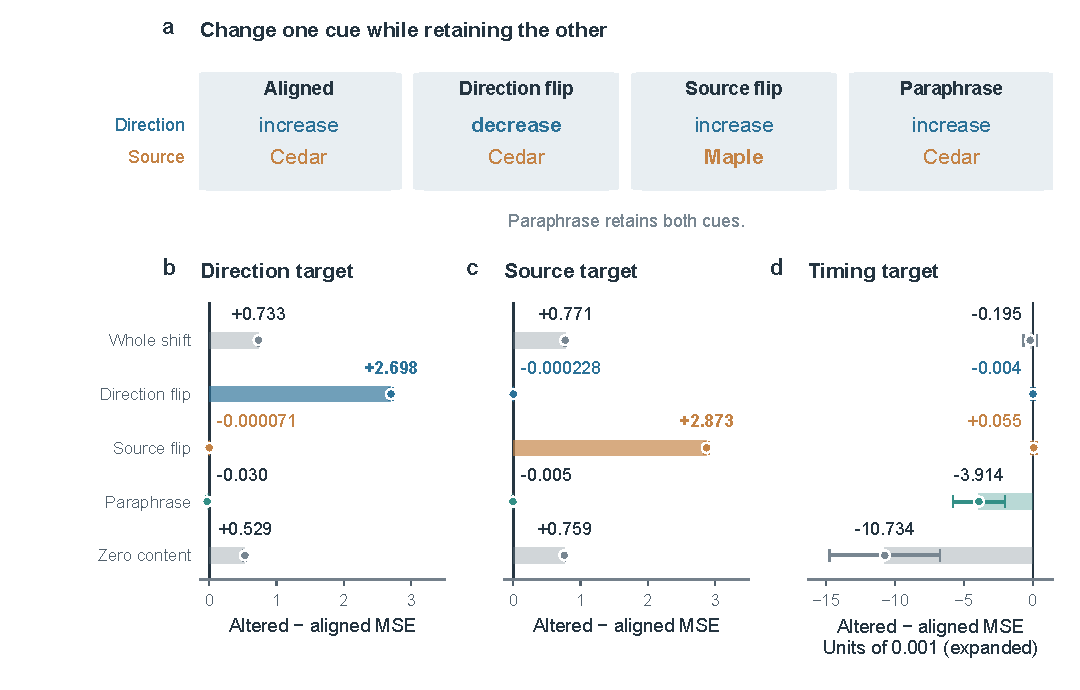
\includegraphics[width=\textwidth]{fig7_construct}
\caption{Selective content edits discriminate the stipulated target cue. (a) Abbreviated direction/source examples show which cue changes; paraphrases change wording while preserving both cues. (b--d) All fifteen fixed-predictor altered-minus-aligned MSE effects for direction, source and timing targets. Points show means and whiskers the saved 95\% $t$ intervals across twenty generated worlds, conditional on shared empirical clocks. Direction and source panels share their scale; the timing axis is expanded in units of 0.001. This contrast concerns the stated cues within the finite generated vocabulary. Table~\ref{tab:construct_full} retains rejection fractions and adverse paraphrase outcomes.}
\label{fig:construct}
\end{figure}
